% !TeX program = pdflatex
% The Staircase of Signs -- Sturm's root-counting theorem in Lean 4.
% Part of the reverse-formalization line (Mathlib gaps -> formalize): after Newton's
% inequalities, Sturm's theorem is the next missing classical result in real-root counting.
% Build: pdflatex sturm-lean.tex (twice, for refs)
% Verified against the Lean source 2026-06-15 (lake env lean Sturm.lean, exit 0;
% #print axioms Sturm.sturm -> propext, Classical.choice, Quot.sound only).
% Toolchain v4.30.0-rc2, Mathlib pin 701fb6e9. Worked example re-checked in exact arithmetic.

\documentclass[11pt]{article}
\usepackage[T1]{fontenc}
\usepackage{lmodern}
\usepackage{amsmath,amssymb,amsthm,booktabs,graphicx,hyperref}
\usepackage{xurl}
\usepackage[table]{xcolor}
\definecolor{ggteal}{HTML}{1B6F8C}
\definecolor{ggband}{HTML}{DCE7EB}
\definecolor{ggamber}{HTML}{E08A1E}
\usepackage[margin=1in]{geometry}
\usepackage{microtype}
\usepackage{float}
\usepackage[section]{placeins}
\usepackage[most]{tcolorbox}
\usepackage{tikz}
\usetikzlibrary{arrows.meta,positioning}
\graphicspath{{figures/}}
\setlength{\emergencystretch}{2em}
\newtheorem{theorem}{Theorem}
\newtheorem{lemma}{Lemma}
\newtheorem{proposition}{Proposition}
\newtheorem{remark}{Remark}
\newcommand{\lean}[1]{\texttt{#1}}
\newcommand{\R}{\mathbb{R}}
\newcommand{\V}{\mathrm{V}}
\hypersetup{colorlinks=true,linkcolor=ggteal,citecolor=ggteal,urlcolor=ggteal}
\newtcbox{\keybox}{on line,boxrule=0.9pt,colframe=ggteal,colback=ggband!40,
  arc=3pt,left=8pt,right=8pt,top=5pt,bottom=5pt}
\newcommand{\keyeq}[1]{\begin{center}\keybox{$\displaystyle #1$}\end{center}}
\newtcolorbox{recipebox}[1]{colframe=ggamber,colback=ggamber!8,arc=3pt,boxrule=0.8pt,
  title=\textbf{#1},coltitle=white,colbacktitle=ggamber}

\title{\bf The Staircase of Signs\\[4pt]
  \large\normalfont Sturm's root-counting theorem, machine-checked in Lean~4}
\author{Carles Mar\'in\thanks{Formalized with the assistance of an AI system (Claude,
Anthropic); the mathematics is Sturm's, and every claim, scope statement, and limitation is
the author's responsibility. The boundary of the contribution is set out plainly in
Section~\ref{sec:boundary}, and the Lean kernel---not the assistant---is what certifies the
proofs.}\\[3pt]
  \normalsize Independent researcher\\
  \normalsize \texttt{karlesmarin@gmail.com}}
\date{June 2026}

\begin{document}
\maketitle

\begin{abstract}
I report a complete, \lean{sorry}-free formalization in Lean~4, over Mathlib, of \emph{Sturm's
theorem} (1829): for a squarefree real polynomial $p$ and an interval $(a,b]$ whose endpoints
are not roots, the number of distinct real roots of $p$ in $(a,b]$ equals
\[
  \V(a)-\V(b),
\]
where $\V(x)$ is the number of sign changes in the \emph{Sturm sequence}
$p,\,p',\,-(p \bmod p'),\,\dots$ evaluated at $x$ (zeros discarded). No root is ever located;
two integers are subtracted. The mathematics is entirely classical and the result has been
formalized before in other systems (Coq, Isabelle/HOL, HOL~Light); to the best of my knowledge
this is the first proof of Sturm's theorem in Lean. The contribution is therefore the
formalization itself and the reusable machinery it required: a small theory of sign variation,
an inductive ``flank-reduction'' relation that decouples the chain's combinatorics from its
algebra, and the local-to-global passage from a single root crossing to the interval count. The
headline theorem \lean{Sturm.sturm} depends only on the three standard axioms \lean{propext},
\lean{Classical.choice}, \lean{Quot.sound}. A by-product is that Mathlib's existing count of
coefficient sign variations (Descartes' rule) and the count used here are, after unfolding,
\emph{the same function}---so the toolkit transfers verbatim to Descartes.
\end{abstract}

\medskip
\noindent\emph{What you will find here.} This is a short guided tour, not a reference manual. It
is organized as four questions, each opening a section and handing the reader the next. The first
asks how two integers can possibly count roots (Section~\ref{sec:q1}); the second, why the count
moves only at the roots, and by exactly one (Section~\ref{sec:q2}); the third, where the proof
genuinely resists being made formal, and what that resistance taught me (Section~\ref{sec:q3});
the fourth, what becomes free once the theorem is in the library (Section~\ref{sec:q4}). The load-
bearing lemmas are gathered in one table (Section~\ref{sec:blocks}, Table~\ref{tab:inventory});
the honest limits---squarefreeness, the ground field, what was \emph{not} proved, and the prior
formalizations in other systems---are stated without varnish in Section~\ref{sec:boundary}; and
the closing section asks, by way of reflection, what this paper still lacks. If you read only two
things, read Theorem~\ref{thm:sturm} and Figure~\ref{fig:staircase}; the rest is the argument that
connects them.

\begin{figure}[h]
\centering
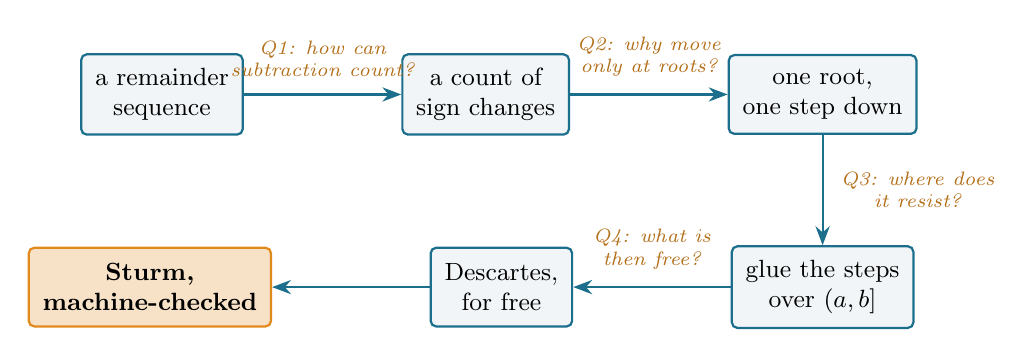
\begin{tikzpicture}[
  obj/.style={draw=ggteal,thick,rounded corners=2pt,fill=ggband!40,align=center,
    font=\small,inner sep=5pt,minimum height=10mm},
  q/.style={font=\scriptsize\itshape,text=ggamber!80!black,align=center},
  arr/.style={-{Stealth[length=2.4mm]},thick,ggteal}]
  \node[obj] (seq) {a remainder\\sequence};
  \node[obj,right=20mm of seq] (count) {a count of\\sign changes};
  \node[obj,right=20mm of count] (quantum) {one root,\\one step down};
  \node[obj,below=14mm of quantum] (glue) {glue the steps\\over $(a,b]$};
  \node[obj,left=20mm of glue] (free) {Descartes,\\for free};
  \node[obj,left=20mm of free,fill=ggamber!25,draw=ggamber] (done)
    {\textbf{Sturm,}\\\textbf{machine-checked}};
  \draw[arr] (seq) -- node[q,above=1mm] {Q1: how can\\subtraction count?} (count);
  \draw[arr] (count) -- node[q,above=1mm] {Q2: why move\\only at roots?} (quantum);
  \draw[arr] (quantum) -- node[q,right=1mm] {Q3: where does\\it resist?} (glue);
  \draw[arr] (glue) -- node[q,above=1mm] {Q4: what is\\then free?} (free);
  \draw[arr] (free) -- (done);
\end{tikzpicture}
\caption{The reader's map. From a sequence of remainders to a certified root count and what it
yields downstream; each arrow is the question its section answers. Every node is a block of
\lean{sorry}-free Lean.}
\label{fig:readermap}
\end{figure}

\section{The question that begins it}\label{sec:intro}

How many real roots does a polynomial have between here and there---and can you say so without
finding a single one of them?

The question is old and was, for a long time, genuinely hard. Descartes' rule of signs
(1637)~\cite{descartes} reads a \emph{bound} off the signs of the coefficients; Budan and Fourier
(early nineteenth century)~\cite{bf} sharpened it to a bound for an interval; but a bound is not a
count, and the gap between them resisted the best analysts of the age. It was closed in 1829 by a
young Charles-Fran\c{c}ois Sturm, who announced---and in 1835 published in full~\cite{sturm}---a
procedure that returns the \emph{exact} number of distinct real roots in any interval, with no
approximation and no root-finding whatsoever. The method was celebrated at once; it is the
ancestor of real-root isolation, of cylindrical algebraic decomposition, and of the decision
procedures for the first-order theory of the reals that grew out of Tarski's work. The problem of
counting real roots exactly was, in effect, settled by a subtraction.

The mechanism is a small twist on something even older. Euclid's algorithm, run on $p$ and its
derivative $p'$, produces a sequence of remainders; Sturm's twist is to negate each remainder as
it is formed,
\[
  p_0=p,\quad p_1=p',\quad p_{k+1}=-(p_{k-1}\bmod p_k),
\]
stopping when the remainder vanishes. Call this the \emph{Sturm sequence}. For a point $x$ that is
not a root of any member, let $\V(x)$ be the number of times the sign changes as one reads
$p_0(x),p_1(x),\dots$ from left to right, ignoring any zeros. Sturm's theorem is the statement
that $\V$ is, in disguise, a root counter:
\keyeq{\#\{\text{distinct real roots of }p\text{ in }(a,b]\}\;=\;\V(a)-\V(b).}

The result is textbook, and has been machine-checked before: in Coq, as part of Cohen's
construction of the real algebraic numbers~\cite{cohen}; in Isabelle/HOL, by Eberl~\cite{eberl}
and---in the sharper Sturm--Tarski form, via the Cauchy index---by Li and
Paulson~\cite{litarski,libudan}; and in HOL~Light. What it had not been, until now, is checked in
\emph{Lean}. Mathlib, the library on which a large part of contemporary formalized mathematics is
built, carries Descartes' rule of signs (the function \lean{Polynomial.signVariations}) but not
Sturm's sequence and not Sturm's theorem. This paper fills that gap. It is, I want to be exact, a
first-in-Lean and not a first-in-any-system; the value is in adding a foundational tool to a
library that lacked it, and in the reusable pieces the proof leaves behind.

I came to it not by setting out to prove Sturm's theorem but by asking, repeatedly, which
classical results a mature library is still missing---and Sturm's, sitting squarely in real-root
counting, was among the most conspicuous absences. The rest of the paper is the road from the
absence to the theorem, told as the four questions a careful reader is likely to ask in turn.

\section{Q1: how can subtracting two integers count roots?}\label{sec:q1}

\emph{History bead.} The sequence and the counting statement are Sturm's
own~(\cite{sturm}; the modern textbook account is Basu--Pollack--Roy~\cite{bpr}). Nothing in
this section is new mathematics; the Lean is in \lean{Sturm.lean}, definitions \lean{sturmSeq}
and \lean{signVarAt}.

Let us make the two ingredients precise. The Sturm sequence is built by the negated Euclidean
recursion above; in Lean it is \lean{sturmSeq p}, a \lean{List} of polynomials produced by an
auxiliary \lean{sturmAux} that recurses on the divisor's degree and terminates because each
remainder has strictly smaller degree. The sign count is
\[
  \V(x)\;=\;\lean{signVarAt (sturmSeq p) x},
\]
defined as the number of sign changes in the list of evaluated signs
$\big(\mathrm{sign}\,p_0(x),\mathrm{sign}\,p_1(x),\dots\big)$ after deleting the zeros. (In the
Lean source the deletion-and-count is phrased with \lean{List.destutter}; an equivalent and more
convenient recursive form, \lean{signChanges}, is proved equal to it and is what the rest of the
development uses.)

\begin{theorem}[Sturm's theorem, in Lean~4; \lean{Sturm.sturm}]\label{thm:sturm}
Let $p$ be a squarefree real polynomial and $a<b$ with $p(a)\ne0$ and $p(b)\ne0$. Then
\keyeq{\V(a)-\V(b)\;=\;\#\{x : a<x\le b,\ p(x)=0\},}
the number of \emph{distinct} real roots of $p$ in the half-open interval $(a,b]$. The statement
is \lean{sorry}-free; \lean{\#print axioms Sturm.sturm} reports only \lean{propext},
\lean{Classical.choice}, \lean{Quot.sound}.
\end{theorem}

That a difference of two integers should equal a count is, on first sight, a small miracle, so it
is worth seeing it happen once by hand.

\emph{A hand-checkable case.} Take $p(x)=x^3-x=x(x-1)(x+1)$, with roots $-1,0,1$. The negated
Euclidean recursion gives the four-term sequence
\[
  p_0=x^3-x,\quad p_1=3x^2-1,\quad p_2=\tfrac{2}{3}x,\quad p_3=1.
\]
Read the signs at the two endpoints of $(-2,2]$:
\[
  \begin{array}{c|cccc|c}
   x & p_0 & p_1 & p_2 & p_3 & \V \\\hline
   -2 & - & + & - & + & 3 \\
   \phantom{-}2 & + & + & + & + & 0
  \end{array}
\]
so $\V(-2)-\V(2)=3-0=3$, exactly the number of roots in $(-2,2]$. Notice that no root was
computed; only signs were read. (Every entry of this table is re-checked in exact arithmetic by
the script accompanying Figure~\ref{fig:staircase}.)

The picture behind the table is the one that names this paper. Plot $\V(x)$ as $x$ sweeps the
line: it is a \emph{staircase}, flat almost everywhere and dropping by one as $x$ passes each root
of $p$ (Figure~\ref{fig:staircase}; Table~\ref{tab:signs} reads it off point by point). Sturm's
theorem is then nothing but reading the total descent of the staircase between $a$ and $b$. The entire difficulty---and the entire content of the next
two sections---is in proving that the staircase has exactly this shape: that it is flat except at
roots, and that each step has height exactly one.

\begin{figure}[t]
\centering
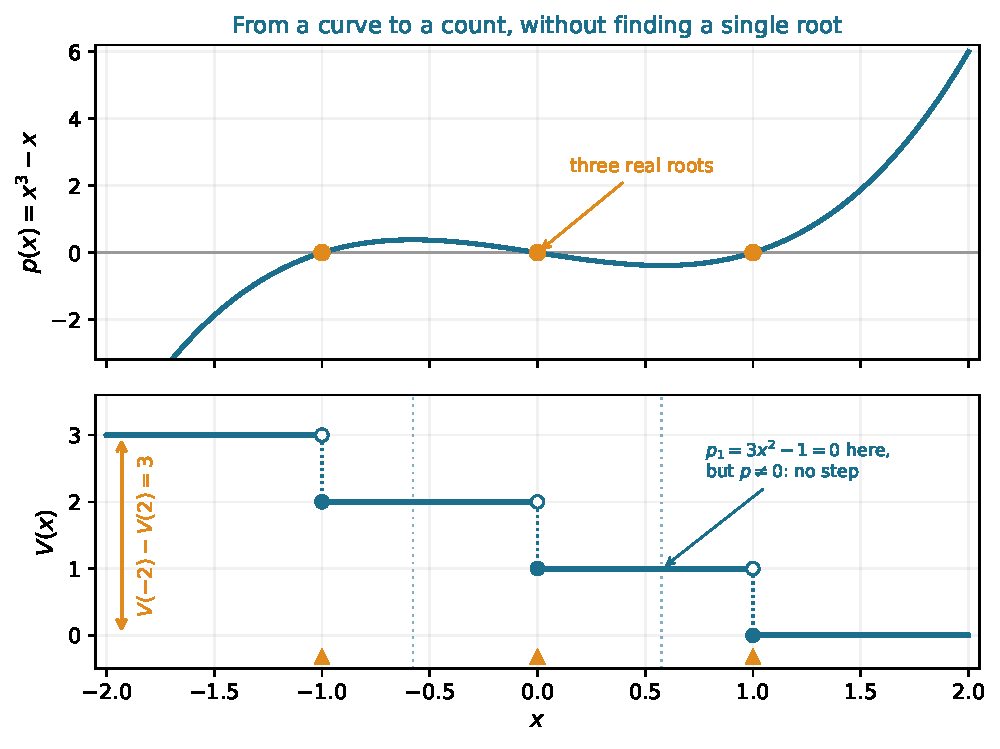
\includegraphics[width=0.93\textwidth]{sturm_fig1_staircase}
\caption{The staircase of signs for $p=x^3-x$. \emph{Top:} the polynomial and its three real
roots. \emph{Bottom:} the count $\V(x)$ is flat except at the roots $-1,0,1$, where it drops by
exactly one (open circle = the value just to the left, filled circle = the value at the root, on
the lower step). At a zero of an \emph{interior} member of the sequence---here $p_1=3x^2-1$
vanishes at $x=\pm1/\sqrt3$ (dotted guides), points where $p$ itself is nonzero---the staircase
does \emph{not} move. The total descent over $(-2,2]$ (the amber arrow) is the number of roots
there. The generating script asserts every plotted sign and count against exact rational
arithmetic before drawing.}
\label{fig:staircase}
\end{figure}

\begin{table}[t]
\centering\small
\rowcolors{2}{ggband!35}{white}
\begin{tabular}{@{}rccccr@{}}
\toprule
\rowcolor{ggteal!18} $x$ & $p_0=x^3{-}x$ & $p_1=3x^2{-}1$ & $p_2=\tfrac23 x$ & $p_3=1$ & $\V(x)$ \\
\midrule
$-2$            & $-$ & $+$ & $-$ & $+$ & $3$ \\
$-1$ {\scriptsize(root)} & $0$ & $+$ & $-$ & $+$ & $2$ \\
$-\tfrac12$     & $-$ & $-$ & $-$ & $+$ & $2$ \\
$-\tfrac{1}{\sqrt3}$ {\scriptsize($p_1{=}0$)} & $-$ & $0$ & $-$ & $+$ & $2$ \\
$0$ {\scriptsize(root)}  & $0$ & $-$ & $0$ & $+$ & $1$ \\
$\tfrac{1}{\sqrt3}$ {\scriptsize($p_1{=}0$)}  & $+$ & $0$ & $+$ & $+$ & $1$ \\
$1$ {\scriptsize(root)}  & $0$ & $+$ & $+$ & $+$ & $0$ \\
$2$             & $+$ & $+$ & $+$ & $+$ & $0$ \\
\bottomrule
\end{tabular}
\caption{The same example read off the signs. Each row evaluates the four chain members and
counts the sign changes (zeros skipped). $\V$ falls by one at each \emph{root} of $p$ and is
unchanged across each zero of the \emph{interior} member $p_1$ (the
$\tfrac{1}{\sqrt3}$ rows)---the two behaviours Section~\ref{sec:q2} explains. The whole table is
regenerated and checked in exact arithmetic by the figure script.}
\label{tab:signs}
\end{table}

\section{Q2: why does the count move only at the roots, and by exactly one?}\label{sec:q2}

\emph{History bead.} The local analysis---what happens to $\V$ as $x$ crosses a point---is the
heart of every proof of Sturm's theorem since Sturm's. The two facts it turns on (a member and
its neighbours cannot vanish together; consecutive members are antipodal at a zero of the one
between them) are classical; the Lean is in the lemmas \lean{not\_common\_root},
\lean{sign\_neighbours\_opposite\_at\_interior\_root}, and
\lean{signVarAt\_drop\_at\_critical\_point}.

Call a point \emph{critical} if some member of the sequence vanishes there. Away from critical
points every member keeps its sign (a polynomial cannot change sign without a root, by the
intermediate value theorem), so $\V$ is locally constant: this is \lean{signVarAt\_eq\_of\_no\_root},
and it is why the staircase is flat between criticals. All the action is at the critical points,
and there are two kinds.

\emph{The roots of $p$.} Suppose $p(c)=0$. Because $p$ is squarefree it shares no root with $p'$,
so $p'(c)\ne0$, and just to the left and right of $c$ the polynomial $p$ takes opposite signs
(it crosses zero transversally, with the sign of $p'(c)$ on the right and the opposite on the
left). The very first pair of the sequence, $(p,p')$, therefore changes its number of internal
sign agreements by exactly one across $c$. This is the single step of the staircase, isolated in
Lean as the leading-pair drop \lean{signVarAt\_cons\_head\_drop}, fed by the transversality lemmas
\lean{sign\_eval\_eq\_sign\_deriv\_right} and \lean{sign\_eval\_eq\_neg\_sign\_deriv\_left}.

\emph{The other critical points.} A member $p_k$ with $1\le k$ may also vanish at $c$ without $p$
doing so. Here is the mechanism that makes Sturm's theorem work, and it is worth stating as the
one indispensable lemma:
\begin{lemma}[antipodal neighbours; \lean{sign\_neighbours\_opposite\_at\_interior\_root}]
\label{lem:antipodal}
If consecutive members $p_{k-1},p_k$ are coprime and $p_k(c)=0$, then $p_{k-1}(c)$ and
$p_{k+1}(c)$ are both nonzero and have \emph{opposite} signs.
\end{lemma}
The reason is a one-line consequence of the defining recursion $p_{k+1}=-(p_{k-1}\bmod p_k)$
evaluated at a root of $p_k$: there $p_{k-1}(c)=-p_{k+1}(c)$ (lemma \lean{eval\_eq\_neg\_next\_of\_root}),
and neither can be zero because coprime polynomials share no root (\lean{not\_common\_root}).
Consequently, whatever sign $p_k$ adopts on either side of $c$---and whether it is positive,
negative, or exactly zero \emph{at} $c$---it sits between two fixed, opposite neighbours, and a
value squeezed between opposite signs contributes nothing to the count of sign changes, regardless
of what it is. The middle member is invisible. This is why a zero of an interior member moves the
staircase not at all (the $p_1=0$ marks in Figure~\ref{fig:staircase}); coprimality of consecutive
members, which propagates along the chain from $\gcd(p,p')=1$, guarantees it everywhere.

Putting the two kinds together gives the per-point quantum---the height of a single step:
\begin{proposition}[single critical point; \lean{signVarAt\_drop\_at\_critical\_point}]
\label{prop:quantum}
If $c$ is the only critical point in $[a,b]$ and $p(a),p(b)\ne0$, then
\[
  \V(a)=\V(b)+\begin{cases}1 & p(c)=0,\\ 0 & p(c)\ne0.\end{cases}
\]
\end{proposition}
The proof is where the formalization earns its keep, and it is the subject of the next section,
because making it rigorous required a device the textbook does not need.

\section{Q3: where does the proof resist being made formal?}\label{sec:q3}

\emph{History bead.} On paper, ``the interior members cancel and only $p$ matters'' is a sentence.
Made formal, it is the one genuinely structural step, because the cancellation has to be performed
\emph{along a list whose shape is itself recursive}. The device that resolves it
(\lean{FlankReduce} and \lean{flankReduce\_chain\_walk}) is, as far as I know, the only part of
this development without a direct textbook antecedent---not a new theorem, but a piece of proof
engineering.

The difficulty is precise. To compare $\V(a)$ with $\V(b)$ across a single critical point $c$, one
wants to delete from the sign list, at \emph{both} $a$ and $b$, every interior member that vanishes
at $c$---each is squeezed between opposite neighbours, so deleting it changes nothing
(Lemma~\ref{lem:antipodal})---and then observe that the two pruned lists differ only in the head
$p$. But ``delete each such member'' is an induction over the Sturm sequence, and the hypotheses
that justify a deletion (the flanking neighbours are nonzero and opposite \emph{at the evaluation
point}) are threaded through the chain's own structure. The combinatorics of pruning a list and the
algebra of why each pruning is legal are entangled, and an honest proof must separate them.

The separation is an inductive relation. Say a list of signs \emph{flank-reduces} to another when
the second is obtained from the first by repeatedly deleting an entry that lies between two nonzero
opposite signs:
\begin{recipebox}{The decoupling (recipe)}
Define \lean{FlankReduce} as the reflexive relation generated by one rule: from
$\textit{pre}\mathbin{+\!\!+}[a,b]\mathbin{+\!\!+}\textit{rest}$ one may pass to
$\textit{pre}\mathbin{+\!\!+}[a,m,b]\mathbin{+\!\!+}\textit{rest}$ whenever $a,b\ne0$ and $a\ne b$.
Two facts then divide the labour cleanly. \emph{Combinatorial:} flank-reduction preserves the
number of sign changes (\lean{FlankReduce.signChanges\_eq})---this is pure list algebra, no
polynomials. \emph{Structural:} the Sturm chain's evaluated sign list at any point flank-reduces to
the chain with its interior $c$-vanishers removed (\lean{flankReduce\_chain\_walk})---this is the
induction over the chain, supplying the flank hypotheses from coprimality and from local sign
constancy, and nothing else.
\end{recipebox}
\begin{figure}[t]
\centering
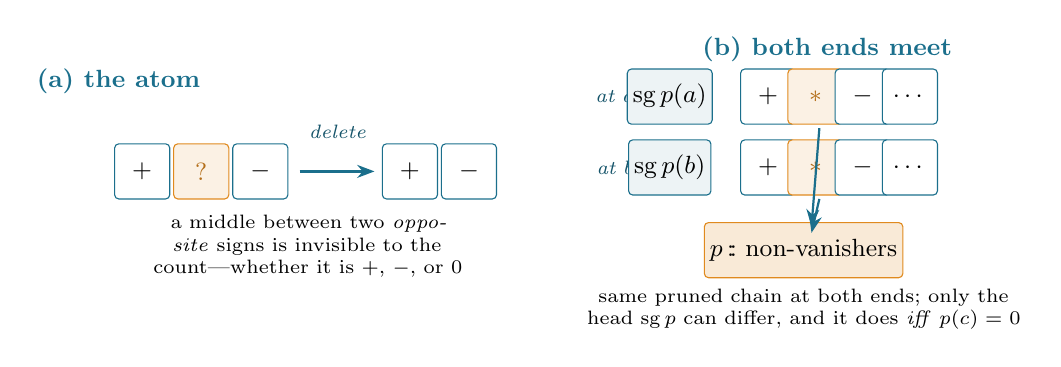
\begin{tikzpicture}[
  s/.style={draw=ggteal,rounded corners=1.5pt,minimum size=7mm,inner sep=2pt,font=\small,fill=white},
  sm/.style={draw=ggamber,rounded corners=1.5pt,minimum size=7mm,inner sep=2pt,font=\small,
    fill=ggamber!12,text=ggamber!80!black},
  arr/.style={-{Stealth[length=2.2mm]},thick,ggteal},
  lbl/.style={font=\scriptsize\itshape,text=ggteal!75!black}]
  % (a) the atom
  \node[font=\bfseries\small,text=ggteal] at (-0.3,1.15) {(a) the atom};
  \node[s] (a1) at (0,0) {$+$};
  \node[sm] (am) at (0.75,0) {$?$};
  \node[s] (a2) at (1.5,0) {$-$};
  \node[s] (b1) at (3.4,0) {$+$};
  \node[s] (b2) at (4.15,0) {$-$};
  \draw[arr] (2.0,0) -- (2.95,0);
  \node[lbl,align=center] at (2.48,0.5) {delete};
  \node[font=\scriptsize,align=center,text width=5.2cm] at (2.1,-0.95)
    {a middle between two \emph{opposite} signs is invisible to the count---whether it is
     $+$, $-$, or $0$};
  % (b) the two reductions meeting
  \node[font=\bfseries\small,text=ggteal] at (8.7,1.55) {(b) both ends meet};
  % at a
  \node[lbl] at (6.05,0.95) {at $a$:};
  \node[s,fill=ggband!50] (pa) at (6.7,0.95) {$\mathrm{sg}\,p(a)$};
  \node[s] at (7.95,0.95) {$+$};
  \node[sm] at (8.55,0.95) {$\ast$};
  \node[s] at (9.15,0.95) {$-$};
  \node[s] at (9.75,0.95) {$\cdots$};
  % at b
  \node[lbl] at (6.05,0.05) {at $b$:};
  \node[s,fill=ggband!50] (pb) at (6.7,0.05) {$\mathrm{sg}\,p(b)$};
  \node[s] at (7.95,0.05) {$+$};
  \node[sm] at (8.55,0.05) {$\ast$};
  \node[s] at (9.15,0.05) {$-$};
  \node[s] at (9.75,0.05) {$\cdots$};
  % reduced
  \node[s,fill=ggamber!18,draw=ggamber] (red) at (8.4,-1.0) {$p\,\mathbin{:\!:}$ non-vanishers};
  \draw[arr] (8.6,0.55) -- (8.5,-0.7);
  \draw[arr] (8.6,-0.35) -- (8.5,-0.78);
  \node[font=\scriptsize,align=center,text width=5.6cm] at (8.4,-1.75)
    {same pruned chain at both ends; only the head $\mathrm{sg}\,p$ can differ, and it does
     \emph{iff} $p(c)=0$};
\end{tikzpicture}
\caption{The decoupling of Section~\ref{sec:q3}. \emph{(a)} The combinatorial atom: an entry
flanked by opposite nonzero signs ($\ast$, the interior vanisher) can be deleted without changing
the number of sign changes, whatever its own value. \emph{(b)} Applied along the chain at both
endpoints, every interior $c$-vanisher is deleted, so the sign lists at $a$ and at $b$ reduce to
the \emph{same} pruned chain; the only entry that can differ is the head $\mathrm{sg}\,p$. The
chain's algebra supplies the ``opposite neighbours'' hypotheses; the count is moved by
\lean{FlankReduce}, which never mentions a polynomial.}
\label{fig:flank}
\end{figure}

With the two halves separated, Proposition~\ref{prop:quantum} becomes assembly: the chain's sign
list flank-reduces, at $a$ and at $b$ alike, to the \emph{same} pruned chain $p\mathbin{:\!:}(\text{non-vanishers})$;
on that pruned chain only $p$ can change sign between $a$ and $b$, so the change in $\V$ is the
single head-drop when $p(c)=0$ and nothing otherwise. The chain structure enters only to hand the
combinatorial lemma its hypotheses; the count is moved by a relation that knows nothing of
polynomials.

\emph{What the machine made me state correctly.} There is a quieter lesson here, of the kind a
proof assistant is good at extracting. The classical proof tacitly assumes ``generic position'':
that no member of the sequence vanishes at the endpoints $a,b$, and that one may always slide to
such points. Formalizing forbids the hand-wave---and it turns out the flank-reduction already
handles the awkward cases for free. A member vanishing exactly at an evaluation point is still
squeezed between opposite neighbours there, so it is still deleted by the same relation; the pruned
chain is the same; the count is unaffected. I therefore proved the per-point lemma
(Proposition~\ref{prop:quantum}) for a critical point anywhere in the closed interval $[a,b]$,
endpoints included, rather than only strictly inside---and the degenerate cases the textbook waves
past are discharged by the same line as the main one. The transferable principle is the same one
the companion paper on Newton's inequalities~\cite{newton} drew: phrasing a step at the weakest
honest level of generality often dissolves, rather than multiplies, the edge cases.

\emph{From one step to the whole staircase.} The global statement is then an induction on the
number of critical points in $(a,b]$ (\lean{Sturm.sturm}; the criticals are the roots of the
product of all members, a nonzero polynomial, hence finite). Peel off the largest critical point
$c$; choose a non-critical separator $d$ just below it---one exists because the criticals are
finite and the reals are dense; apply the per-point quantum on $[d,b]$, where $c$ is the only
critical point; and recurse on $[a,d]$, which has one fewer. The half-open interval $(a,b]$ splits
as $(a,d]\sqcup(d,b]$, the root count adds, and the per-point contribution---one when $p(c)=0$,
zero otherwise---matches the number of $p$-roots in the peeled piece. The global count is assembled
from the per-point steps.

\begin{remark}[the pattern behind \lean{FlankReduce}]\label{rem:pattern}
\lean{FlankReduce} is worth abstracting from its use here. It is an instance of a recurring schema:
a numerical invariant---the sign-change count---preserved under deletions that are licensed by a
purely \emph{local} side-condition (an entry between two opposite nonzero signs). One might call this
a \emph{count invariant under admissible pruning}. Its value is precisely the decoupling exhibited
above: the global combinatorics reduces to (i)~a one-step preservation lemma, polynomial-free and
proved once (\lean{FlankReduce.signChanges\_eq}), and (ii)~a structural walk that certifies each
deletion's side-condition from the problem at hand (\lean{flankReduce\_chain\_walk}). The same
separation should apply wherever a tally is invariant under locally-justified removals---the
derivative sequence of Budan--Fourier, or more generally any rewriting system with a conserved count.
I prove only the instance Sturm needed and do not develop the general theory; but the shape is
general, and naming it---rather than inlining the deletions into the chain induction---is what made
the proof modular. Whether ``invariance of a tally under locally-licensed deletion'' deserves to be
a Mathlib abstraction in its own right is the open question I find most worth carrying forward
(Section~\ref{sec:questions}).
\end{remark}

\section{Q4: what becomes free once the theorem is certified?}\label{sec:q4}

\emph{History bead.} Sturm's count of \emph{interval} sign variations and Descartes' count of
\emph{coefficient} sign variations (1637) are usually taught as cousins. In Lean they turn out to
be, after unfolding, the very same function---a small surprise the formalization surfaced for free.
The Lean is \lean{signVariations\_eq\_signChanges}.

Mathlib already had Descartes' rule of signs, phrased through \lean{Polynomial.signVariations}, the
number of sign changes in a polynomial's coefficient list. The count built here for Sturm's theorem,
\lean{signChanges}, is defined on an arbitrary list of signs. Unfolding both, they coincide on the
nose:
\keyeq{\lean{P.signVariations}\;=\;\lean{signChanges}\,(\lean{P.coeffList.map sign}),}
a proof that is literally \lean{rfl}. The consequence is practical: the toolkit assembled for
Sturm---zeros are invisible to the count, an entry between opposite neighbours cancels, the head
recursion, the parity (a zero-free list has an even number of sign changes iff its ends agree)---is
not Sturm-specific. It transfers verbatim to Descartes, and the two classical sign-variation
theorems now share a single combinatorial core in the library rather than two parallel ones. A
small unification, but exactly the kind a formal library should accumulate.

Two further things fall out without new work. First, \emph{root isolation}: applying the theorem to
$(a,b]$ and to its two halves repeatedly isolates each real root in an interval as small as one
likes, the algorithmic use Sturm's method is best known for. Second, the \emph{building blocks}
themselves---local sign constancy, the antipodal-neighbour lemma, the structural facts about the
sequence (consecutive members coprime, the recursion relating each triple, the final member a
nonzero constant)---are reusable for any further work on real-root counting in Lean: the
Budan--Fourier theorem, the Sturm--Tarski count with multiplicity~\cite{libudan}, or a Cauchy-index
development would draw on the same pieces.

\section{What a certified root count enables}\label{sec:enables}

The mathematics here is two centuries old; the reason to put it in Lean is what it unlocks
\emph{inside} the library, where a verified, exact root count had simply not existed. It is worth
being concrete about that, because a foundational lemma is valuable in proportion to what rests on
it. Four things become reachable that were not before, in rough order of distance from what is
proved.

\emph{Real-root isolation.} The classical algorithmic use of Sturm's theorem is to isolate each
real root in an interval as narrow as desired: apply the count to $(a,b]$, bisect, recurse, and
stop a branch when its count is $0$ (no root) or $1$ (exactly one). Because the count here is
\emph{exact}, not a bound, the recursion provably terminates with one root per interval. Every
ingredient is already proved---the count, local constancy, the finiteness of the critical
set---so what remains is the recursive wrapper and its termination, not new mathematics. This turns
the theorem from a statement into a certified \emph{procedure}, the form in which Sturm's method is
actually used.

\emph{The Budan--Fourier theorem.} Budan and Fourier count sign variations in the sequence of
\emph{derivatives} $p,p',p'',\dots$ and bound (with the right parity) the roots in an interval.
That is the same sign-variation arithmetic as here, on a different sequence; the toolkit built for
Sturm---zeros invisible, the head recursion, and in particular the parity lemma
\lean{wallCount\_even\_iff\_endpoints}---transfers directly. Mathlib already had Descartes' rule
(\lean{signVariations}); Budan--Fourier sits between Descartes and Sturm, and the pieces to reach
it are now in place.

\emph{Sturm--Tarski and the Cauchy index.} The sharper Sturm--Tarski theorem counts roots of $p$
\emph{weighted} by the sign of a second polynomial $q$ on them---the ``Tarski query''---through the
Cauchy index of $q'p/q$ (or $p'q/p$). This is the engine of root counting \emph{with
multiplicity}, of the non-squarefree case, and ultimately of Tarski's quantifier elimination for
the reals. The signed-remainder sequence and the sign-variation count assembled here are precisely
its substrate; the Isabelle development of Sturm--Tarski~\cite{litarski,libudan} is built on the
same two objects. A Lean version would extend, not restart, the present file.

\emph{Decision procedures over the reals.} One-dimensional real-root counting and isolation are the
base case of cylindrical algebraic decomposition and of the decision procedures for the first-order
theory of real-closed fields (Tarski--Seidenberg). For Lean specifically this is the missing
foundation under any future \emph{certified} answer to ``does this polynomial have a root in this
range, and how many''---a checkable certificate a downstream tactic could trust, rather than an
oracle it must believe. None of these four is done here; the point is that each was blocked, in
Lean, on exactly the result this paper supplies.

\section{The building blocks}\label{sec:blocks}

The theorem rests on a handful of reusable lemmas, each \lean{sorry}-free with the standard three
axioms (Table~\ref{tab:inventory}). Three are worth naming for their portability beyond Sturm.

\begin{lemma}[local sign constancy; \lean{signVarAt\_eq\_of\_no\_root}]
If no member of the sequence has a root in $[a,b]$, then $\V(a)=\V(b)$.
\end{lemma}
The intermediate value theorem, lifted from one polynomial to the list: this is the flatness of the
staircase between critical points, and the engine of the global induction's base case.

\begin{lemma}[flank-reduction preserves the count; \lean{FlankReduce.signChanges\_eq}]
If a sign list flank-reduces to another, the two have the same number of sign changes.
\end{lemma}
The combinatorial half of Section~\ref{sec:q3}, depending on no polynomial at all---the cleanest
statement of ``entries between opposite neighbours do not matter.''

\begin{lemma}[the chain's structure; \lean{sturmAux\_consecutive\_coprime}, \lean{sturmAux\_consecutive\_succ}, \lean{sturmAux\_getLast\_isUnit}]
Consecutive members of the sequence are coprime; each consecutive triple satisfies
$p_{k+1}=-(p_{k-1}\bmod p_k)$; and the last member is a nonzero constant.
\end{lemma}
These three facts, proved by induction on the defining recursion, are exactly what
Lemma~\ref{lem:antipodal} and the global induction consume.

\begin{table}[h]
\centering\small
\rowcolors{2}{ggband!35}{white}
\begin{tabular}{@{}lll@{}}
\toprule
\rowcolor{ggteal!18} Lean name & statement & role \\
\midrule
\lean{Sturm.sturm} & $\V(a)-\V(b)=\#\{a<x\le b:p(x)=0\}$ & Theorem~\ref{thm:sturm} \\
\lean{sturmSeq} & the negated signed-remainder sequence & definition \\
\lean{signVarAt} & sign changes of the list evaluated at $x$ & definition \\
\lean{signVarAt\_drop\_at\_critical\_point} & per-point quantum $\Delta\V\in\{0,1\}$ & Prop.~\ref{prop:quantum} \\
\lean{flankReduce\_chain\_walk} & chain reduces to its non-vanishers & the wall (\S\ref{sec:q3}) \\
\lean{FlankReduce.signChanges\_eq} & flank-reduction preserves the count & combinatorial core \\
\lean{sign\_neighbours\_opposite\_at\_interior\_root} & antipodal neighbours at a zero & Lemma~\ref{lem:antipodal} \\
\lean{signVarAt\_cons\_head\_drop} & a head sign-flip raises $\V$ by one & root crossing \\
\lean{signVarAt\_eq\_of\_no\_root} & $\V$ constant off the critical set & constancy \\
\lean{sturmAux\_consecutive\_coprime} & consecutive members coprime & structure \\
\lean{sturmAux\_consecutive\_succ} & $p_{k+1}=-(p_{k-1}\bmod p_k)$ & structure \\
\lean{sturmAux\_getLast\_isUnit} & last member a nonzero constant & structure \\
\lean{signVariations\_eq\_signChanges} & $=$ Descartes' count (by \lean{rfl}) & bridge (\S\ref{sec:q4}) \\
\bottomrule
\end{tabular}
\caption{The load-bearing results, all \lean{sorry}-free in \lean{Sturm.lean}. The axioms of every
entry are \lean{propext}, \lean{Classical.choice}, \lean{Quot.sound} only; no \lean{native\_decide},
no custom axiom.}
\label{tab:inventory}
\end{table}

How those results depend on one another is easier to see as a tree than as a list
(Figure~\ref{fig:deptree}): the theorem splits into the per-point quantum and the constancy on the
gaps, the quantum into the flank-reduction and the single head-drop, and the flank-reduction into
its pure count-invariance and the antipodal-neighbour fact---with the structural facts feeding the
global induction underneath.

\begin{figure}[h]
\centering
\begin{tcolorbox}[colframe=ggteal,colback=ggband!18,arc=2pt,boxrule=0.7pt,left=8pt,right=8pt,
  top=5pt,bottom=5pt,width=\textwidth]
\ttfamily\footnotesize
Sturm.sturm \ \ \ \ \ \ \ \ \ \ \ \ \ \ \ \ \ \ \ \ \ \ (global induction on the critical set)\\
\ |-- signVarAt\_drop\_at\_critical\_point \ \ (per-point quantum, Sec.~\ref{sec:q2})\\
\ | \ \ \ |-- flankReduce\_chain\_walk \ \ \ \ \ \ (prune interior c-vanishers)\\
\ | \ \ \ | \ \ \ |-- FlankReduce.signChanges\_eq \ (count invariant)\\
\ | \ \ \ | \ \ \ `-- sign\_neighbours\_opposite...\ (antipodal neighbours)\\
\ | \ \ \ |-- signVarAt\_cons\_head\_drop \ \ \ \ \ (the single step, p(c)=0)\\
\ | \ \ \ `-- signVarAt\_eq\_of\_no\_root \ \ \ \ \ \ (no step, p(c)$\neq$0)\\
\ |-- signVarAt\_eq\_of\_no\_root \ \ \ \ \ \ \ \ \ \ (flat gaps between criticals)\\
\ `-- sturmAux\_consecutive\_\{coprime,succ\} \ (chain structure)\\
\ \ \ \ \ \ + sturmAux\_getLast\_isUnit
\end{tcolorbox}
\caption{The dependency tree of \lean{Sturm.sturm}. Reading top to bottom is reading
Sections~\ref{sec:q1}--\ref{sec:q3} in reverse: the pure, polynomial-free
\lean{FlankReduce.signChanges\_eq} at the bottom, the Sturm-specific assembly at the top.}
\label{fig:deptree}
\end{figure}

\subsection*{Cost and reuse}

Because a formalization is judged as much by its cost as by its conclusion, here is the
development measured (Table~\ref{tab:cost}). The whole proof is a single file, \lean{Sturm.lean},
of about $1{,}220$ lines: $54$ lemmas and theorems, $5$ definitions, and one inductive relation.
It depends on Mathlib alone---twelve modules, listed in the source---and on nothing from the
earlier papers in this line; it is self-contained over the library. On a pre-built Mathlib it
checks in about nine seconds (Lean \lean{v4.30.0-rc2}), so the iteration loop during development
was tight. The reuse is worth quantifying rather than estimating. Of the roughly $1{,}165$ lines
inside declarations, about $220$ are \emph{pure} sign/list combinatorics that mention no polynomial
at all (\lean{signChanges}, \lean{wallCount}, \lean{FlankReduce} and the list-surgery lemmas)---the
layer that transfers verbatim to Descartes (Section~\ref{sec:q4})---and a further $\approx 200$ are
general polynomial sign-variation lemmas, reusable for any real-root sign argument. The genuinely
Sturm-specific remainder is about $750$ lines: the sequence's structure and the local-to-global
crossing. So roughly a third of the development outlives its original purpose.

\begin{table}[h]
\centering\small
\rowcolors{2}{ggband!35}{white}
\begin{tabular}{@{}l p{0.62\textwidth}@{}}
\toprule
\rowcolor{ggteal!18} measure & value \\
\midrule
Lean source & \lean{Sturm.lean}, $\approx 1{,}220$ lines, one file \\
declarations & $54$ lemmas/theorems, $5$ definitions, $1$ inductive \\
dependencies & Mathlib only ($12$ modules); none on prior work \\
compile time & $\approx 9$\,s (file only, against a pre-built Mathlib), Lean \lean{v4.30.0-rc2} \\
axioms & \lean{propext}, \lean{Classical.choice}, \lean{Quot.sound} \\
line split & $\approx 220$ pure sign/list combinatorics $+$ $\approx 200$ general polynomial sign-variation (both reusable) $+$ $\approx 750$ Sturm-specific \\
\bottomrule
\end{tabular}
\caption{The development measured. The compile time is for checking \lean{Sturm.lean} against a
Mathlib that is already built; building Mathlib itself is the usual one-time cost and is not part of
the contribution. The line split is counted from the declaration bodies (comments and blank lines
excluded).}
\label{tab:cost}
\end{table}

\section{The boundary of the contribution}\label{sec:boundary}

Let me be as plain about the limits as about the result.

\emph{The mathematics is Sturm's.} I claim no new theorem and no new method. The sequence, the
counting statement, the local crossing analysis, and the reduction to a difference of sign counts
are all classical (Sturm~\cite{sturm}; the modern treatment in Basu--Pollack--Roy~\cite{bpr}). The
contribution is the formalization, together with the reusable infrastructure---the sign-variation
toolkit, the \lean{FlankReduce} decoupling, the structural facts about the sequence---that any
further real-root development in Lean would want.

\emph{Scope, stated plainly.} I prove the theorem for \emph{squarefree} $p$. This is the standard
normalization and loses no generality in principle: for arbitrary $p$ one passes to
$p/\gcd(p,p')$, which is squarefree with the same distinct roots---but I have \emph{not} formalized
that reduction here, so the squarefree hypothesis is a genuine boundary of what is checked, not
merely a convenience. I work over $\R$, the natural home of the result and what the
intermediate-value and transversality arguments use, not over an abstract real-closed field. The
endpoints are assumed non-roots of $p$; tail members \emph{may} vanish at the endpoints, and that
case is handled (Section~\ref{sec:q3}). I count \emph{distinct} roots; for squarefree $p$ distinct
and with-multiplicity coincide, so no separate multiplicity statement is needed, but neither is the
Sturm--Tarski count with sign-weighted multiplicities~\cite{litarski,libudan} attempted.

\emph{Where this sits, as a contribution.} Judged as pure mathematics the novelty is essentially
nil---Sturm's theorem is from 1829. Judged as a formalization it is, I think, worth recording: a
foundational classical result genuinely absent from a major library, proved in full with reusable
infrastructure and one piece of non-obvious engineering. The natural readership is the formalized-
mathematics and verification community rather than the pure-mathematical one, and I have tried to
write for it---hence the cost accounting, the reuse analysis, and the comparison that follows.

\emph{Prior formalizations, and what differs across systems.} The priority claim is narrow and
rests on a documented search, not a feeling. Sturm's theorem has been formalized before: in Coq,
within Cohen's construction of the real algebraic numbers~\cite{cohen}; in Isabelle/HOL by
Eberl~\cite{eberl} (a standalone development with an executable \lean{sturm} proof method) and, in
the sharper Sturm--Tarski form via the Cauchy index, by Li and Paulson~\cite{litarski,libudan}; and
in HOL~Light. What I searched for (June~2026) and did not find was any formalization of the Sturm
sequence or Sturm's theorem in \emph{Lean}/Mathlib (Loogle and \lean{grep}:
\lean{Polynomial.signVariations} for Descartes' rule exists; no \lean{sturm}, no signed-remainder
sequence). So: first in Lean, to the best of my knowledge; not first in any system.

A word on what the choice of system cost and saved, since that is what a proof-engineering reader
will want. What Mathlib \emph{gave}, and made several steps almost free: the Euclidean-domain
identity $p = (p\div q)\,q + (p\bmod q)$ with the degree bound $\deg(p\bmod q)<\deg q$, which makes
the sequence's definition terminate without a separate measure argument; \lean{Polynomial.Splits},
\lean{roots} and \lean{mem\_roots'} for the root set; \lean{separable} together with
\lean{PerfectField.separable\_iff\_squarefree}, which delivers ``squarefree $\Rightarrow$ coprime to
the derivative'' in one line; the intermediate value theorem (\lean{intermediate\_value\_Icc}); and
\lean{Finset.max'} with the cardinality lemmas for the global induction. The analytic and algebraic
substrate, in other words, was already there. What was \emph{absent everywhere in Lean} and had to
be built is the sign-variation theory and the whole local-to-global crossing argument; and the one
genuinely fiddly step---independent of the system---was the list-recursion coupling that
\lean{FlankReduce} resolves (Section~\ref{sec:q3}), not the analysis. I did not port Cohen's or
Eberl's proofs, so I make no claim about relative proof length or difficulty: a fair comparison
would mean re-doing the work in each system, which I have not done. What I can say is that the
approaches differ in setting---Cohen's is embedded in exact-real-arithmetic, Eberl's is executable,
Li--Paulson's targets the Cauchy index---and that, in Lean, the cost lived in the combinatorics of
the count, not in the polynomial analysis Mathlib already supports.

\emph{On method.} The formalization was carried out with an AI assistant (Claude, Anthropic), under
the discipline used throughout this line of work: the worked example verified in exact arithmetic
before formalizing (the script behind Figure~\ref{fig:staircase}), and every named theorem checked
by \lean{\#print axioms} to rest only on \lean{propext}, \lean{Classical.choice}, \lean{Quot.sound}.
Correctness does not depend on the assistant: the Lean kernel checks every proof, and a reader who
trusts the kernel need trust nothing else. The careful accounting in this section---the squarefree
boundary named as a boundary, the prior systems credited---is part of what the method, used
honestly, should produce.

\section{What this paper still lacks}\label{sec:questions}

Sturm's theorem is now in the library; the more interesting question is what its absence was hiding,
and what this account leaves undone. I close with the questions I would rather carry forward than
pretend to have settled---each a place where the present work stops short.

\begin{enumerate}\itemsep3pt
\item \emph{The squarefree boundary.} I leaned on squarefreeness and did not formalize the passage
to $p/\gcd(p,p')$. That reduction is routine on paper; is it routine in Lean, or does the gcd of a
polynomial and its derivative hide the kind of degree-bookkeeping that, as in
Section~\ref{sec:q3}, only looks routine until a machine asks? Closing it would make the theorem
unconditional, and is the first thing I would do next.

\item \emph{The two counts, beyond \lean{rfl}.} Descartes' and Sturm's variation counts turned out
to be the same function (Section~\ref{sec:q4}). That is a coincidence of \emph{definition}; is there
a theorem behind it---a single statement of which Descartes' bound and Sturm's exact count are two
instances, and which a library could hold once instead of twice? The shared core is suggestive, but
I have only unified the bookkeeping, not the theorems.

\item \emph{From count to certificate.} The proof says \emph{how many} roots lie in $(a,b]$; it does
not, as it stands, hand back the roots themselves, nor a checkable certificate of the count for a
skeptical downstream tool. The building blocks for root isolation are all here
(Section~\ref{sec:q4}); what is the smallest honest bridge from this theorem to a verified
root-isolation procedure---and how much of Sturm--Tarski~\cite{libudan} would it want along the way?

\item \emph{What the decoupling really is.} The \lean{FlankReduce} relation separated the
combinatorics of pruning a list from the algebra of why each pruning is legal
(Section~\ref{sec:q3}). It worked cleanly enough that I suspect it is an instance of something more
general---a pattern for any argument where a count is invariant under deletions licensed by local
side-conditions. Is ``invariance of a tally under locally-justified deletion'' a reusable lemma in
its own right, or did it merely happen to fit here? I do not yet know, and that uncertainty is the
honest state of it.
\end{enumerate}

\section*{Reproducing}
\begin{verbatim}
git clone https://github.com/karlesmarin/godsil-gutman-lean
cd godsil-gutman-lean && lake exe cache get
lake env lean Sturm.lean
\end{verbatim}
Lean \lean{v4.30.0-rc2}, Mathlib pin \lean{701fb6e9}. The theorem is \lean{Sturm.sturm} in
\lean{Sturm.lean}; its supports are in Table~\ref{tab:inventory}. It is checked by \lean{\#print
axioms} to depend only on \lean{propext}, \lean{Classical.choice}, \lean{Quot.sound}. The
worked example of Figure~\ref{fig:staircase} is re-derived, and every sign and count asserted
against exact rational arithmetic, before the figure is drawn.

\begin{thebibliography}{99}\small
\bibitem{descartes} R.~Descartes, \emph{La G\'eom\'etrie} (1637); the rule of signs bounds the
number of positive roots by the number of sign changes of the coefficients.
\bibitem{bf} F.~D.~Budan de Boislaurent, \emph{Nouvelle m\'ethode pour la r\'esolution des
\'equations num\'eriques} (1807); J.~Fourier, \emph{Analyse des \'equations d\'etermin\'ees}
(posth.\ 1831). The Budan--Fourier theorem bounds the roots in an interval by a sign-variation
difference.
\bibitem{sturm} C.~Sturm, M\'emoire sur la r\'esolution des \'equations num\'eriques,
\emph{M\'emoires pr\'esent\'es par divers savants \`a l'Acad\'emie Royale des Sciences} \textbf{6}
(1835) 271--318; presented to the Acad\'emie in 1829.
\bibitem{bpr} S.~Basu, R.~Pollack, M.-F.~Roy, \emph{Algorithms in Real Algebraic Geometry}, 2nd
ed., Algorithms and Computation in Mathematics \textbf{10}, Springer, 2006 (Sturm's theorem and
sign-variation theory, Ch.~2).
\bibitem{cohen} C.~Cohen, Construction of real algebraic numbers in Coq, in \emph{Interactive
Theorem Proving (ITP 2012)}, LNCS \textbf{7406}, Springer, 2012, 67--82.
\bibitem{eberl} M.~Eberl, Sturm's Theorem, \emph{Archive of Formal Proofs} (2014),
\url{https://isa-afp.org/entries/Sturm_Sequences.html}.
\bibitem{litarski} W.~Li, L.~C.~Paulson, A formal proof of the Sturm--Tarski theorem,
\emph{Archive of Formal Proofs} (2014), \url{https://isa-afp.org/entries/Sturm_Tarski.html}.
\bibitem{libudan} W.~Li, The Budan--Fourier theorem and counting real roots with multiplicity,
preprint, 2018, \texttt{arXiv:1811.11093}; see also W.~Li, G.~O.~Passmore, L.~C.~Paulson, Deciding
univariate polynomial problems using untrusted certificates in Isabelle/HOL, \emph{J.~Automated
Reasoning} \textbf{62} (2019) 69--91.
\bibitem{mathlib} The mathlib Community, The Lean mathematical library, in \emph{Certified Programs
and Proofs (CPP 2020)}, ACM, 2020, 367--381.
\bibitem{gglean} C.~Mar\'in, \emph{Random Signs into Matchings: A Godsil--Gutman Identity,
Formalized in Lean~4}, Zenodo, 2026, \texttt{doi:10.5281/zenodo.20517350}.
\bibitem{newton} C.~Mar\'in, \emph{The Inward Bow of a Real-Rooted Polynomial: Newton's
Inequalities, Machine-Checked in Lean~4}, Zenodo, 2026, \texttt{doi:10.5281/zenodo.20693064}.
\end{thebibliography}

\end{document}
